\documentclass[tikz,border=10pt]{standalone}
\usetikzlibrary{positioning}
\usepackage{tkz-graph}
\usepackage{rotating}
\usetikzlibrary{arrows}
\usetikzlibrary{arrows.meta}

\begin{document}
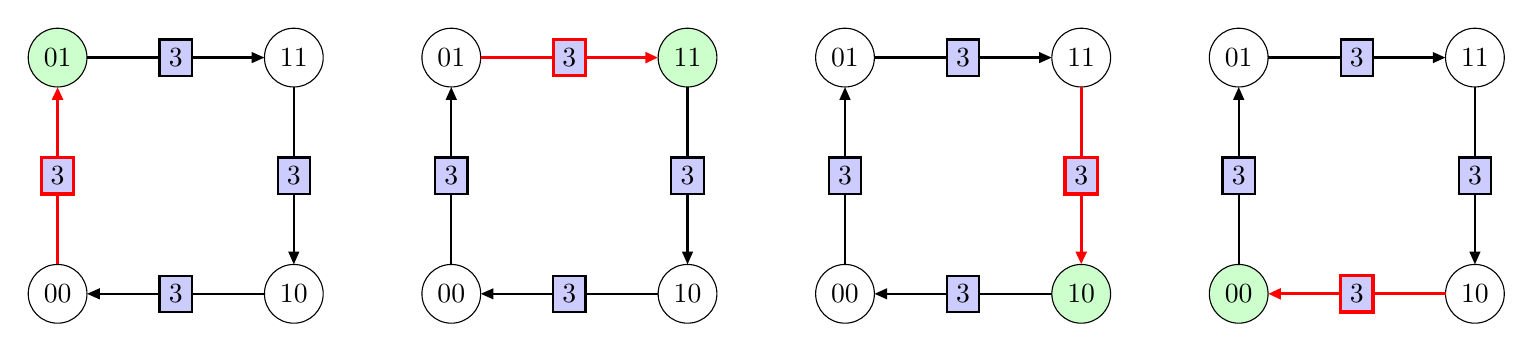
\begin{tikzpicture}
\SetGraphUnit{3}
\GraphInit[vstyle=Dijkstra]
\tikzset{LabelStyle/.style= {draw, fill = blue!20}}
\tikzset{VertexStyle/.style = {shape = circle, fill = green!20, draw}}
\Vertex {01}
\tikzset{VertexStyle/.style = {shape = circle, fill = white, draw}}
\EA(01){11} 
\SO(11){10}
\WE(10){00}
\Edges[style={-{Triangle[angle=45:5pt]}}, label=$3$](01,11)
\Edges[style={-{Triangle[angle=45:5pt]}}, label=$3$](11,10)
\Edges[style={-{Triangle[angle=45:5pt]}}, label=$3$](10,00)
\SetUpEdge[style={draw=red,very thick,-{Triangle[angle=45:5pt]}}]
\tikzset{LabelStyle/.style ={draw,fill=blue!20}}
\Edges[label=$3$](00,01)
\begin{scope}[xshift=5cm]
\SetGraphUnit{3}
\GraphInit[vstyle=Dijkstra]
\tikzset{LabelStyle/.style= {draw,
fill = blue!20}}
\Vertex {01}
\tikzset{VertexStyle/.style = {shape = circle, fill = green!20, draw}} 
\EA(01){11}
\tikzset{VertexStyle/.style = {shape = circle, fill = white, draw}}
\SO(11){10} 
\WE(10){00}
\Edges[style={-{Triangle[angle=45:5pt]}}, label=$3$](11,10)
\Edges[style={-{Triangle[angle=45:5pt]}}, label=$3$](10,00)
\Edges[style={-{Triangle[angle=45:5pt]}}, label=$3$](00,01)
\SetUpEdge[style={draw=red,very thick,-{Triangle[angle=45:5pt]}}]
\tikzset{LabelStyle/.style ={draw,fill=blue!20}}
\Edges[label=$3$](01,11)
\end{scope}
\begin{scope}[xshift=10cm]
\SetGraphUnit{3}
\GraphInit[vstyle=Dijkstra]
\tikzset{LabelStyle/.style= {draw,
fill = blue!20}}
\Vertex {01}
\EA(01){11} 
\tikzset{VertexStyle/.style = {shape = circle, fill = green!20, draw}} 
\SO(11){10}
\tikzset{VertexStyle/.style = {shape = circle, fill = white, draw}}
\WE(10){00}
\Edges[style={-{Triangle[angle=45:5pt]}}, label=$3$](10,00)
\Edges[style={-{Triangle[angle=45:5pt]}}, label=$3$](00,01)
\Edges[style={-{Triangle[angle=45:5pt]}}, label=$3$](01,11)
\SetUpEdge[style={draw=red,very thick,-{Triangle[angle=45:5pt]}}]
\tikzset{LabelStyle/.style ={draw,fill=blue!20}}
\Edges[label=$3$](11,10)
\end{scope}
\begin{scope}[xshift=15cm]
\SetGraphUnit{3}
\GraphInit[vstyle=Dijkstra]
\tikzset{LabelStyle/.style= {draw, fill = blue!20}}
\Vertex {01}
\EA(01){11}
\SO(11){10}
\tikzset{VertexStyle/.style = {shape = circle, fill = green!20, draw}} 
\WE(10){00}
\Edges[style={-{Triangle[angle=45:5pt]}}, label=$3$](00,01)
\Edges[style={-{Triangle[angle=45:5pt]}}, label=$3$](01,11)
\Edges[style={-{Triangle[angle=45:5pt]}}, label=$3$](11,10)
\SetUpEdge[style={draw=red,very thick,-{Triangle[angle=45:5pt]}}]
\tikzset{LabelStyle/.style ={draw,fill=blue!20}}
\Edges[label=$3$](10,00)
\end{scope}
\end{tikzpicture}
\end{document}